\documentclass[10pt,pdf,hyperref={unicode}, dvipsnames]{beamer}
\usepackage[english,russian]{babel}
% \usepackage[T2A,T1]{fontenc}
\usepackage[utf8]{inputenc}
\usepackage{tikz}
\usepackage[unicode]{hyperref}
\usepackage{pgfplots,standalone}
\usepackage
	{
		% Дополнения Американского математического общества (AMS)
		amssymb,
		amsfonts,
		amsmath,
		amsthm,
		physics
		}
% \usepackage{lmodern}
\pgfplotsset{compat=newest} 
\usetikzlibrary{%
    decorations.pathreplacing,%
    decorations.pathmorphing,%
    patterns,%
    angles,%
    quotes,%
    calc, %
    3d, %
    backgrounds, %
    positioning%
}


% Стиль презентации

 \usetheme{Warsaw}
 \usefonttheme{professionalfonts}
 \usecolortheme{}
 % \usecolortheme{whale}

 

% \setbeamercolor{frametitle right}{fg=white,bg=Brown!85}
% \setbeamercolor{frametitle}{fg=white,bg=Brown!85}
% \setbeamercolor{frametitle right}{fg=white,bg=black!85} %
\setbeamercolor{frametitle}{fg=white,bg=black!85} % Цвет титульника

\setbeamertemplate{headline}{}
\setbeamertemplate{footline}{}
\let\Tiny=\tiny % решает проблему со шрифтами в TexLive
\setbeamertemplate
	{footline}{
		\color{black!40!white}
		\quad\hfill
		\insertframenumber/\inserttotalframenumber
		\hfill\vspace{1cm}\quad
	} 

\setbeamertemplate{navigation symbols}{}

\beamersetrightmargin{1cm} 
\beamersetleftmargin{1cm}

\setbeamertemplate{enumerate item}{
	\usebeamercolor[bg]{item projected}
	\raisebox{1pt}{\colorbox{bg}{\color{fg}\footnotesize\bf\insertenumlabel}}%
}
\setbeamercolor{item projected}{bg=black,fg=white}


\setbeamertemplate{itemize item}{%
	\usebeamercolor[bg]{item projected}%
	\raisebox{1pt}{{\color{bg}\footnotesize$\bf\square$}}%
}
\setbeamercolor{item projected}{bg=black,fg=white}
\setbeamercolor{title}{bg=black,fg=white}
\renewcommand{\phi}{\varphi}
\renewcommand{\epsilon}{\varepsilon}
\renewcommand{\div}{\operatorname{div}}
\title[Измерение плотности плазмы]{Измерение плотности плазмы на  экспериментальном стенде КРОТ зондом с СВЧ-резонатором}

\author{%
	Виноградов И.Д. %
	Понур К.А. %
	Шиков А.П. %
}

\institute{Радиофизический факультет ННГУ, 430 группа}

\date{Нижний Новгород, 2018}

\begin{document}  
\begin{frame}
\titlepage
\end{frame}
% \begin{frame}
% \tableofcontents
% \end{frame}
\section{Введение}
\subsection{Цели работы}
\begin{frame}[t]
	\frametitle{Цели работы}
	% \textbf{Цели}\\
		\vfill
		\begin{enumerate}
			% \item \sout{Получить зачёт по УНЭ.}
			\item Изучить принцип работы зонда с СВЧ-резонатором.

			\item Измерить зависимость локальной концентрации плазмы			от расстояния до центра генерации.

			\item Изучить временную зависимость концентрации для распадающейся плазмы.

		\end{enumerate}
		\vfill
\end{frame}
\subsection{Актуальность работы}
\begin{frame}[t]

	
	\frametitle{Актуальность работы}
		\vfill
		\begin{enumerate}
			\item Изучение космического окружения Земли. Например, изучение ионосферы.
			\item Современная астрофизика. Например, для предсказания хода эволюции галактик применялась кинетическая теория плазмы.
			% \item Идея управляемого термоядерного синтеза
			\item МГД-преобразование энергии и ионные двигатели.
			\item Накачка газового лазера газовым разрядом.
			\item Газоразрядные электронные приборы.
		\end{enumerate}


\end{frame}

\section{Краткая теория}
\subsection{Некоторые свойства плазмы}
% \begin{frame}
% 	\frametitle{Некоторые свойства плазмы}
% 	\textbf{Плазма} -- частично или полностью ионизированный газ, образованный из нейтральных атомов (или молекул) и заряженных частиц.

% 	$\,$
% 	\begin{enumerate}
% 		\item Квазинейтральный газ
% 		\item Экранирует действующие на неё на неё электрические поля
% 		\item Высокая проводимость
% 		% \item 
% 	\end{enumerate}
% 	Плазма является электрически нейтральной системой.
% \end{frame}

\begin{frame}[t]\frametitle{Радиус Дебая}
\begin{minipage}[0.5\textheight]{\textwidth}

	\begin{columns}[T]

		\begin{column}{0.4\textwidth}
			\begin{figure}[tb]
				\vspace{0pt}
				\centering
				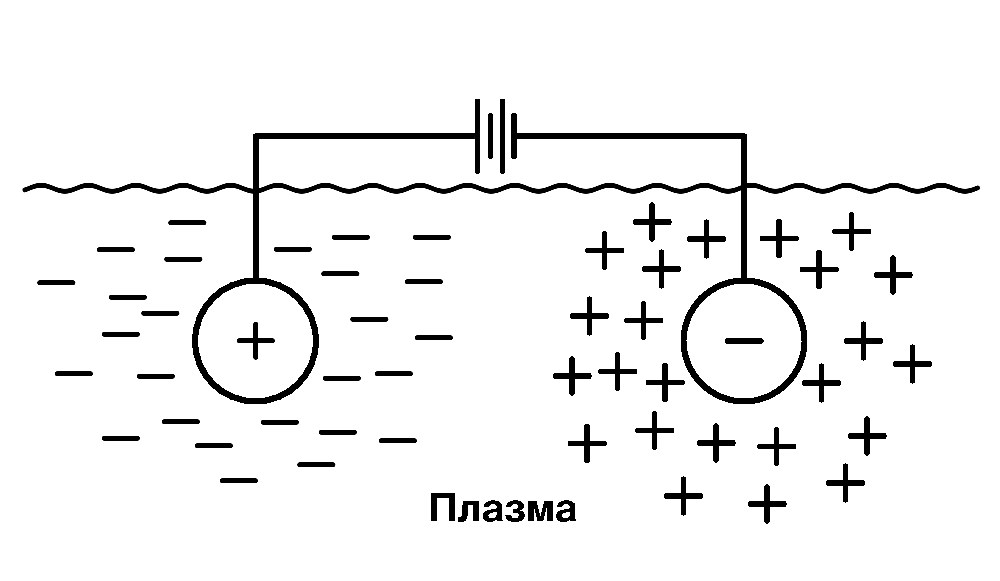
\includegraphics[width=\textwidth]{fig/debai}
				\label{fig:debai}
				\vspace{-20pt}

				\caption*{Дебаевское экранирование}

			\end{figure}
		\end{column}


		\begin{column}{0.6\textwidth}
			Предположим, что мы попытались создать электрическое поле внутри плазмы, поместив в неё два шарика, соединив их батарейкой. Рассмотрим пространство вокруг положительно заряженного  иона.

			Электрическое поле $\vec{E}$ и плотность электрического заряда $\rho$ связаны соотношением:

		\end{column}
	\end{columns}
\end{minipage}

\begin{equation}
	\div{\vec{E}}=4\pi \rho
\end{equation}
\begin{equation}
	\Delta\phi= -4\pi\rho,\, \Delta \text{-- оператор Лапласа}
\end{equation}

	Распределение электронов,
	а значит, и их пространственного заряда
$\rho_e$ описывается формулой Больцмана:
\begin{equation}
	\rho_e= Ne\cdot \exp{-e\phi/kT_e}.
\end{equation}



\end{frame}
\begin{frame}[t]\frametitle{Радиус Дебая (продолжение)}
	\begin{equation}
	\label{eq:1}
	\dv[2]{\phi}{t}+\frac2r\dv{\phi}{r}=-4\pi Ne\left[1 -\exp{-e\phi/kT_e}\right]
\end{equation}
При $\displaystyle \frac{e\phi}{kT_e}\ll1$ можем разложить экспоненту в ряд и (\ref{eq:1}) станет линейным:
\begin{equation}
	\label{eq:2}
	\dv[2]{\phi}{t}+\frac2r\dv{\phi}{r}=\frac{1}{r_D^2}\phi,
\end{equation}
где $\displaystyle r_D^2=\frac{kT_e}{4\pi Ne^2}$.
	Тогда, решение (\ref{eq:2}) имеет вид 
	\begin{equation}
		\label{eq:3}
		\phi=\frac{A_0}{r}\cdot e^{-r/r_D}
	\end{equation}  
    Решение уравнения (\ref{eq:3}) показывает, что поле иона убывает с расстоянием экспоненциально с характерной длиной, равной $r_D$ -- дебаевскому радиусу экранирования. 

    \vfill
    Плазму можно считать  \textbf{квазинейтральной} в областях, размеры которых существенно превосходят дебаевскую длину.
\end{frame}
\begin{frame}[t]\frametitle{Плазменная частота}
\begin{minipage}[0.2\textheight]{\textwidth}
	\begin{columns}[T]
%Без учета магнитного поля
		\begin{column}{0.4\textwidth}
			\begin{figure}[tr]
				\vspace{0pt}
				\centering
				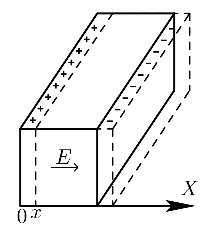
\includegraphics[]{fig/plasmfreq}
				\vspace{-10pt}
				\label{fig:plasmfreq}
				\caption*{Объем, занимаемый ионами обозначен сплошной линией, а электронами -- пунктирной.}
			\end{figure}
		\end{column}


		\begin{column}{0.6\textwidth}
			Сместим все электроны на $x$ относительно ионов. Тогда на гранях выделенного нами параллелепипеда возникнут поверхностные заряды:
			\begin{equation}
			\sigma = Nex,
			\end{equation}
			где $N$-- концентрация электронов
			\begin{equation}
				E=4\pi\sigma=4\pi Nex
			\end{equation}
			Это поле действует на электроны, придавая им ускорение, равное
			\begin{equation}
				\label{eq:4}
				\dv[2]{x}{t}=\frac{eE}{m_e}=\frac{4\pi N e^2}{m_e}x
			\end{equation}
		\end{column}

	\end{columns}
\end{minipage}
\vfill
Уравнение (\ref{eq:4}) определяет плазменную частоту коллективных колебаний электронов:
\begin{equation}
	\omega_p=\sqrt{\frac{4\pi N e^2}{m_e}}
\end{equation}



\end{frame}


\subsection{Зонд с СВЧ-резонатором} % (fold)

\begin{frame}
	\frametitle{Зонд с СВЧ-резонатором}
	Идея метода замера локальной  плотности плазмы заключается в измерении собственной частоты резонатора, помещенного в неё.



	В нашем случае резонатором является четвертьволновый отрезок двупроводной линии (четвертьволновый резонатор), замкнутый на одном конце и разомкнутый на другом. 
	\begin{figure}[H]
			\centering
			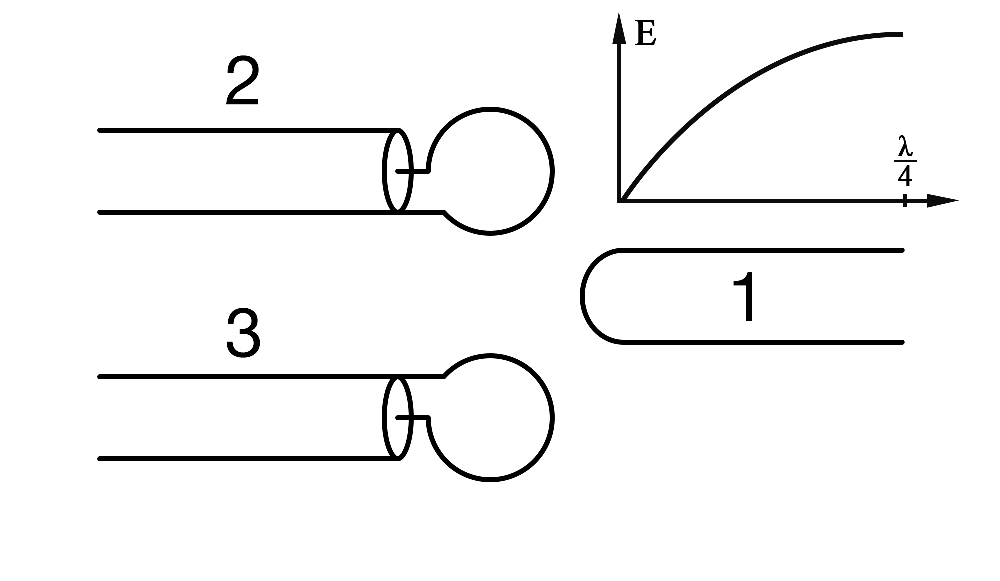
\includegraphics[width=0.8\linewidth]{fig/resonator}
			\caption*{Четвертьволновый резонатор\alert{(1-? 2-? 3-?)}}
			\label{fig:resonator}
	\end{figure}
	

\end{frame}


\begin{frame}
	\frametitle{Зонд с СВЧ-резонатором}

	\begin{equation}
		\omega_{res}=\left(\frac\pi{2l}\right)\frac c{\sqrt{\varepsilon}},
	\end{equation}
	где $\omega_{res}$-- собственная частота резонатора.

	В плазме: $$\varepsilon=\varepsilon(\omega)=1-\frac{\omega^2}{\omega_p^2}.$$ 
	Тогда сдвиг резонансной частоты по сравнению с вакуумом:
	$$\omega_{res}^2=\omega_{0res}^2+\omega_p^2,$$ 
	где $\omega_{0res}$-- собственная частота резонатора в вакууме,а $\omega_p$-- плазменная частота

	При этом концентрация однозначно связана с плазменной частотой:
	\begin{equation}
		N=\frac{m_e\omega^2_p}{4\pi e^2}
	\end{equation}
	% Таким образом мы сможем найти концентрацию.
\end{frame}


\begin{frame}
	\frametitle{Зонд с СВЧ-резонатором}
	\begin{figure}[H]
			\centering
			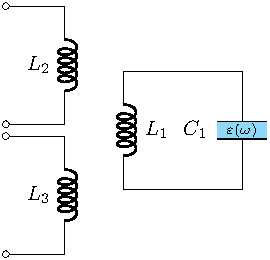
\includegraphics[width=.65\linewidth]{chem/chem1}
			\caption*{Эквивалентная схема резонатора}
			\label{fig:chem1}
	\end{figure}
\end{frame}

\begin{frame}
	\frametitle{Недостатки зонда с СВЧ-резонатором}
	\begin{enumerate}
		\item Контактный метод измерения приводит к возмущению некоторой области около зонда. Характерный размер такой области определяется дебаевским радиусом экранирования и, как правило, оказывается существенно меньше размеров плазменного объема.
		\item Нелинейные свойства и гистерезисные явления. При сильных СВЧ-полях плазма вытесняется из области между проводами резонатора.
	\end{enumerate}
\end{frame}

\begin{frame}
	\frametitle{Преимущества зонда с СВЧ-резонатором}
	\begin{enumerate}
		\item Позволяет определять локальное, слабовозмущенное значение плотности плазмы. 
		\item В сравнении с ленгмюровскими зондами, результаты измерений с помощью зонда с СВЧ-резонатором не зависят в допустимых пределах от электронной температуры плазмы. %узнать как ленгмюровскими мерить плотность

	\end{enumerate}
\end{frame}
% \begin{frame}[t]\frametitle{Нелинейные свойства СВЧ-резонатора}
    


% \end{frame}
\subsection{Генерация плазмы}
\section{Эксперимент}
\subsection{Описание экспериментальной установки}
\begin{frame}
	\frametitle{Экспериментальная установка КРОТ}
	% \begin{block}{Параметры КРОТа}
	Размеры камеры: диаметр 3 м, длина 10 м.

	Размеры соленоида: длина 3.5 м, диаметр 2 м. 
	
	Магнитное поле достигает величины $B\approx 1000$ Эрстед. 
	
	Предельный вакуум, достигаемый в объеме камеры $P =3\cdot10^{-6}$ Торр. 
	% \end{block}
	\begin{figure}[tb]
		\vspace{0pt}
		\centering
		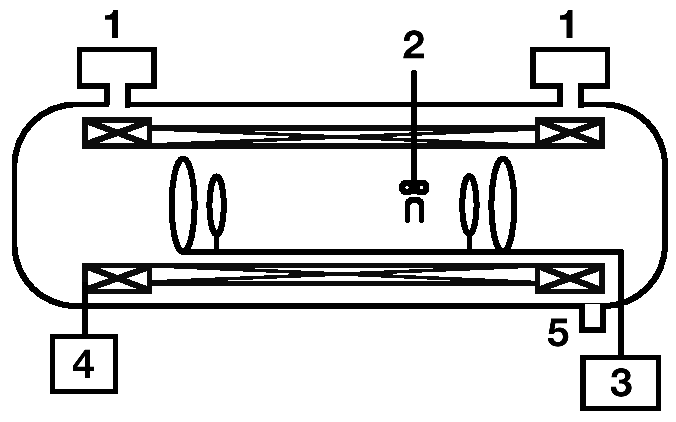
\includegraphics[width=0.6\linewidth]{fig/krot}
		\label{fig:krot}
		\caption*{1 - вакуумная откачка, 2 - зонд с СВЧ-резонатором,3 - ВЧ-генератор, 4 - соленоид с источником магнитного поля, 5 - напуск рабочего газа.}
	\end{figure}
\end{frame}
\begin{frame}
	\frametitle{Генерация плазмы в КРОТе}

		Для генерации плазмы используется индукционный газовый разряд, осуществляемый при помощи высокочастотных вихревых электрических
	полей, создаваемых катушками индуктивности, расположенными внутри установки.
	\begin{figure}[H]
		\begin{minipage}{\linewidth}
				\centering
				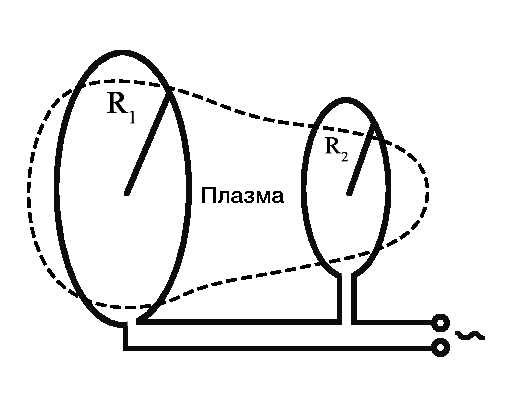
\includegraphics[width=0.4\linewidth]{fig/induct}
				\caption*{Генерация ВЧ поля}
				\label{fig:resonator}
		\end{minipage}
		\end{figure}
\end{frame}
\section{Практическая часть} % (fold)
% \subsection{Измерение концентрации плазмы}
% \begin{frame}
% 	\frametitle{Измерение концентрации плазмы}
% 	Рабочий газ -- аргон (Ag), 
% 	$P=4\cdot10^{-4}$ Торр. 
% 	\begin{figure}[tb]
% 		\vspace{-5pt}
% 		\centering
% 		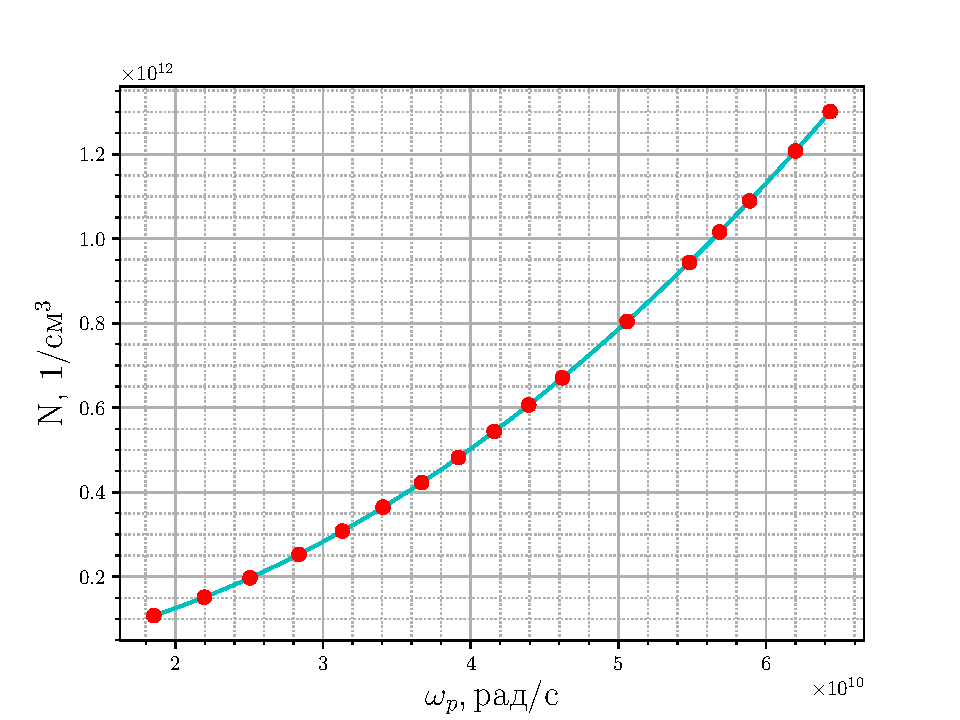
\includegraphics[width=0.89\linewidth]{fig/concentration}
% 		\label{fig:1}
% 	\end{figure}
% \end{frame}
\subsection{Распад  плазмы}
\begin{frame}
	\frametitle{Распад плазмы}
	Из графика определили характерное время распада $\tau_N=4.4$ мс.

	\begin{figure}[tb]
		\centering
		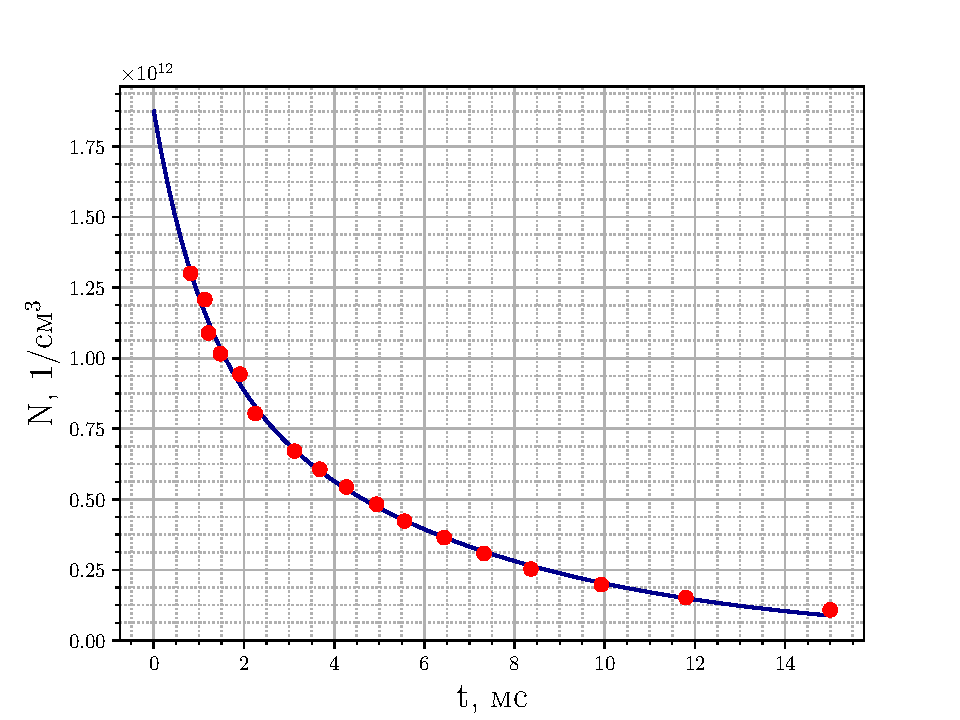
\includegraphics[width=0.9\linewidth]{fig/decay}
		\label{fig:2}
	\end{figure}
\end{frame}

\subsection{Зависимость на радиальной оси}
\begin{frame}
	\frametitle{Зависимость на радиальной оси}
	Время после отключения ВЧ-генератора $t=4.13$ мс
	\begin{figure}[tb]
		\centering
		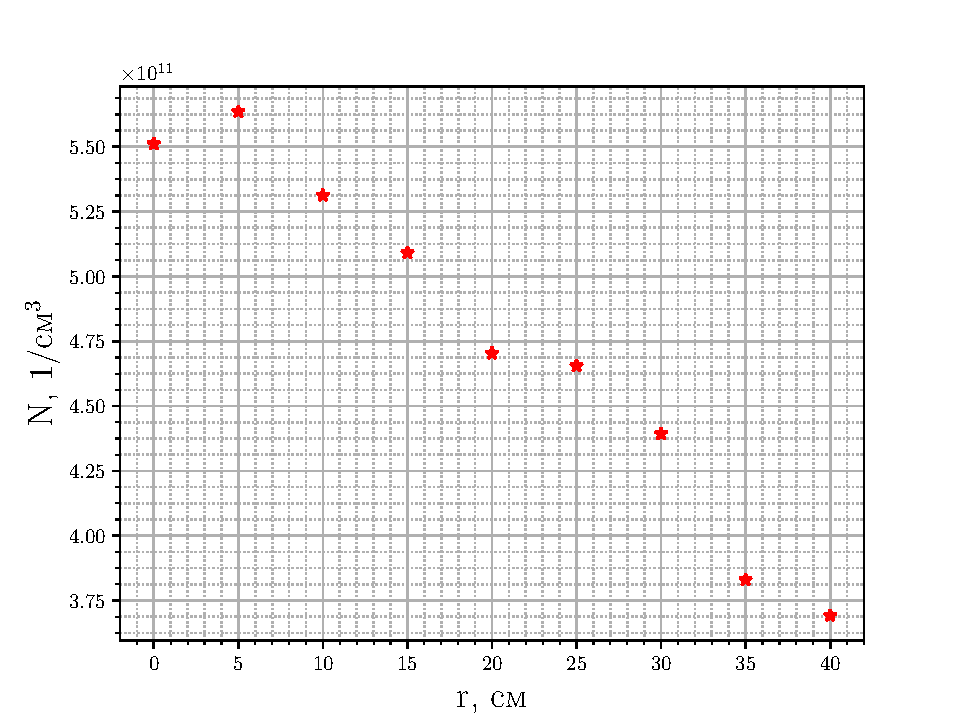
\includegraphics[width=0.9\linewidth]{fig/radial}
		\label{fig:2}
	\end{figure}
\end{frame}

\subsection{Выводы}
\begin{frame}
		\vfill
		\frametitle{Выводы}
		\begin{enumerate}
			\item Был изучен принцип работы зонда с СВЧ-резонатором
			

			\item Была измерена локальная концентрация плазмы в зависимости 
			от удалённости до её центра генерации

			\item А также, снята временная зависимость концентрации для распадающейся плазмы  

		\end{enumerate}
		\vfill
\end{frame}




\end{document}